\documentclass[11pt]{article}   % tipo de documento e tamanho das letras

% os seguintes pacotes estendem a funcionalidade básica:
\usepackage[a4paper, total={16cm, 24cm}]{geometry} % tamanho da pagina e do texto
\usepackage[portuguese]{babel}  % traduz para portugues
\usepackage[utf8]{inputenc}
\usepackage{graphicx}           % graficos
\usepackage{amsmath}            % matematica
\usepackage{tikz}               % diagramas
    \usetikzlibrary{shadows}
\usepackage{booktabs}           % tabelas com  melhor aspecto
\usepackage[colorlinks=true]{hyperref}           % links para partes do documento ou para a web
\usepackage{listings}           % incluir codigo
    \renewcommand\lstlistingname{Listagem}  % Listing em portugues
    \lstset{numbers=left, numberstyle=\tiny, numbersep=5pt, basicstyle=\footnotesize\ttfamily, frame=tb,rulesepcolor=\color{gray}, breaklines=true}
\usepackage{blindtext}

% -------------------------------------------------------------------------------------------
\title
{
    
\includegraphics[width=0.3\textwidth]{images/logo_universidade.png}
    \\[0.1cm]
    \textbf{1ª Parte Trabalho Final} \\
    Metodologias e Desenvolvimento de Software
}

\author
{
    \textbf{Professores:} Pedro Patinho e Pedro Salgueiro \\
    \textbf{Realizado por:} João Pereira (42864) \\ Miguel de Carvalho (43108) \\ Rui Cachapa (37617)
}
\date{\today}

% -------------------------------------------------------------------------------------------
%                                Body                                                       %
% -------------------------------------------------------------------------------------------

\begin{document}
\maketitle

% -------------------------------------------------------------------------------------------
\section{Introdução} 

\hspace{0,5cm}Neste trabalho foi solicitado a realização de um sistema automático de registo de presenças nas aulas de MDS.

% -------------------------------------------------------------------------------------------
\section{Descrição e Planeamento do Sistema}

\subsection{Requisitos do Utilizador}

\begin{itemize}
    \item O Software fornecerá registos das presenças (dos alunos e professores) nas aulas de MDS; 
    \item O Software permite editar os horários das aulas (data, hora, duração e tipo das aulas);
    \item O Software contabiliza a presença dos alunos e dos docentes através da passagem dos cartões;
    \item O Software deve permitir consultar e alterar o estado das faltas (justificadas ou injustificadas);
    \item O Software deve gerar um relatório das faltas dos alunos e das aulas não lecionadas por cada professor, no final do semestre.
\end{itemize}

\subsection{Requisitos do Sistema}

\begin{itemize}
    \item O Sistema deve importar a lista de alunos inscritos nas cadeiras a partir do SIIUE;
    \item Quando o docente não passa o seu cartão, considera-se que não existiu aula e não são contabilizadas as faltas;
    \item Quando um aluno atingir 25 e 50 por cento de aulas não assistidas, o sistema deve enviar um email ao aluno e outro aos docentes a informar sobre esta situação;
    \item Se um aluno passar o cartão depois de decorrida 1h desde o inicio da aula, apenas será considerada meia presença;
    \item A cada hora de aula, o sistema deve avaliar as condições acima, enviando automaticamente os emails necessários;
    \item A qualquer momento, o docente poderá alterar o estado de faltas (justificadas ou injustificadas);
    \item No final do semestre é gerado um relatório com a seguinte informação:
    \begin{itemize}
        \item Lista de alunos com o número de presenças e a respectiva percentagem;
        \item Gráfico de presenças por aula;
        \item Lista de alunos com entre 25 e 50 (por cento) de faltas;
        \item Lista de alunos com mais de 50 (por cento) de faltas;
    \end{itemize}
\end{itemize}

\subsection{Use Cases}

\subsubsection{Login} 

\begin{itemize}
    \item Nome: \textbf{Login}
    \item Ator principal: Aluno, Docente
    \item Comportamento normal de sucesso:
    \begin{enumerate}
        \item Preencher Username, Password
        \item Clicar no botão de Login
        \item mostrar página do programa
    \end{enumerate}
    \item Extenções
    \begin{itemize}
        \item 2 - conta não encontrada:
        \begin{itemize}
            \item Username não encontrado
            \item Password Inválida
        \end{itemize}
        \item 3 - Página de acordo com o Utilizador
        \begin{itemize}
            \item Aluno apenas pode consultar
            \item Professor pode alterar presenças nas sua cadeira
        \end{itemize}
\end{itemize}
    
\subsubsection{Consulta das Presenças}
    
    \item Ator principal: Aluno, Docente
    \item Comportamento normal de sucesso:
    \begin{enumerate}
        \item Preencher Username, Password
        \item Clicar no botão de Login
        \item mostrar página do programa
    \end{enumerate}
    \item Extenções
    \begin{itemize}
        \item 2 - conta não encontrada:
        \begin{itemize}
            \item Username não encontrado
            \item Password Inválida
        \end{itemize}
        \item 3 - Página de acordo com o Utilizador
        \begin{itemize}
            \item Aluno apenas pode consultar
            \item Professor pode alterar presenças nas sua cadeira
        \end{itemize}
    \end{itemize}
\end{itemize}


\subsubsection{Justificar/Injustificar as presenças} 

\begin{itemize}
    \item Ator principal: Professor
    \item Comportamento normal de sucesso:
    \begin{enumerate}
        \item Preencher Username, Password
        \item Clicar no botão de Login
        \item Mostrar página do programa
        \item Selecionar a visualização de presenças
        \item Altera a presença das aulas que desejar
    \end{enumerate}
    
\end{itemize}

\subsubsection{Gerar Relatório} 

\begin{itemize}

    \item Ator principal: Professor
    \item Comportamento normal de sucesso:
    \begin{enumerate}
  
        \item  Preencher Username, Password
        \item Clicar no botão de **Login**
        \item Mostrar página principal do programa
        \item Clicar no botão de **Gerar Relatório**
        \item Envio de um ficheiro PDF sobre as faltas dos alunos para o email do docente.

    \end{enumerate} 

\end{itemize}

\subsubsection{Criação/Alteração do Horário de Funcionamento} 

\begin{itemize}
    \item Ator principal: Professor
    \item Comportamento normal de sucesso:
    \begin{enumerate}
  
        \item Preencher Username, Password
        \item Clicar no botão de **Login**
        \item Mostrar página principal do programa
        \item Clicar no botão **Horários**
        \item Clicar no botão **Editar**
        \item Inserir/alterar os Horarios da disciplina (dias de semana e horas)
        \item Clicar no botão **Apply**
    \end{enumerate} 
\end{itemize}
  
\subsubsection{Sincronização do Membros com o SIIUE} 

\begin{itemize}

    \item Ator principal: Professor
    \item Comportamento normal de sucesso:
    \begin{enumerate}
  
        \item Preencher Username, Password
        \item Clicar no botão de **Login**
        \item Mostrar página principal do programa
        \item Clicar no botão **Alunos**
        \item Clicar no botão **Sincronizar com o SIIUE**
    \end{enumerate} 
\end{itemize}

\subsection{User Stories}
\begin{itemize}
    \item O João é um aluno exemplar, ele passa o cartão no início da aula, tendo a sua presença marcada.
    \item O Miguel é um aluno desatento, não passou o cartão no início da auala e só se lembrou passado 1h de aula. O Miguel decidiu falar com o professor e o professor decide alterar o valor da presença para 1.
    \item O Rui acha-se espertinho, ele passa o cartão no início da aula e vai-se embora. O professor vê este compotamente e decide injustificar a presença, isto é, colocar o valor a 0.
    \item O Rui passa o cartão no início da aula e assiste apenas a 1H da aula, o professor observa este comportamento e muda o valor da presença para metade 0,5.
    \item Um funcionário da UE insere o horário
    \item No início de cada aula o sistema coloca a assiduidade de cada aluno com a seguinta expressão: \verb|n_aulas_assistidas * n_aulas_total * 100|. Caso o resultado seja inferior a 50 por cento, o sistema envia um email de aviso para o respetivo aluno.
    \item Se o professor faltar à aula, não serão contabilizadas as faltas
    \item Caso o professor se esqueça de passar o cartão no início da aula, o sistema irá pensar que o professor faltou e as faltas não serão contabilizadas. Deverá então justificar a sua falta e a dos alunos
    \item No final do semestre, o professor irá receber um relatório gerado pelo sistema.
\end{itemize}

\newpage

\section{Diagramas UML}

\subsection{Diagrama de UseCases}
    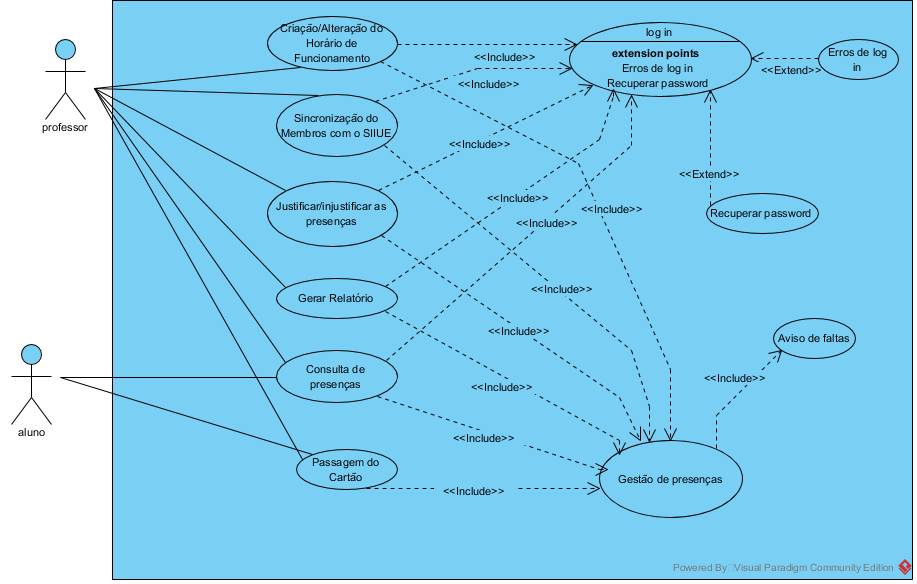
\includegraphics[width=\textwidth]{images/diagra_usecases.png}

\subsection{Diagrama de Classes}
    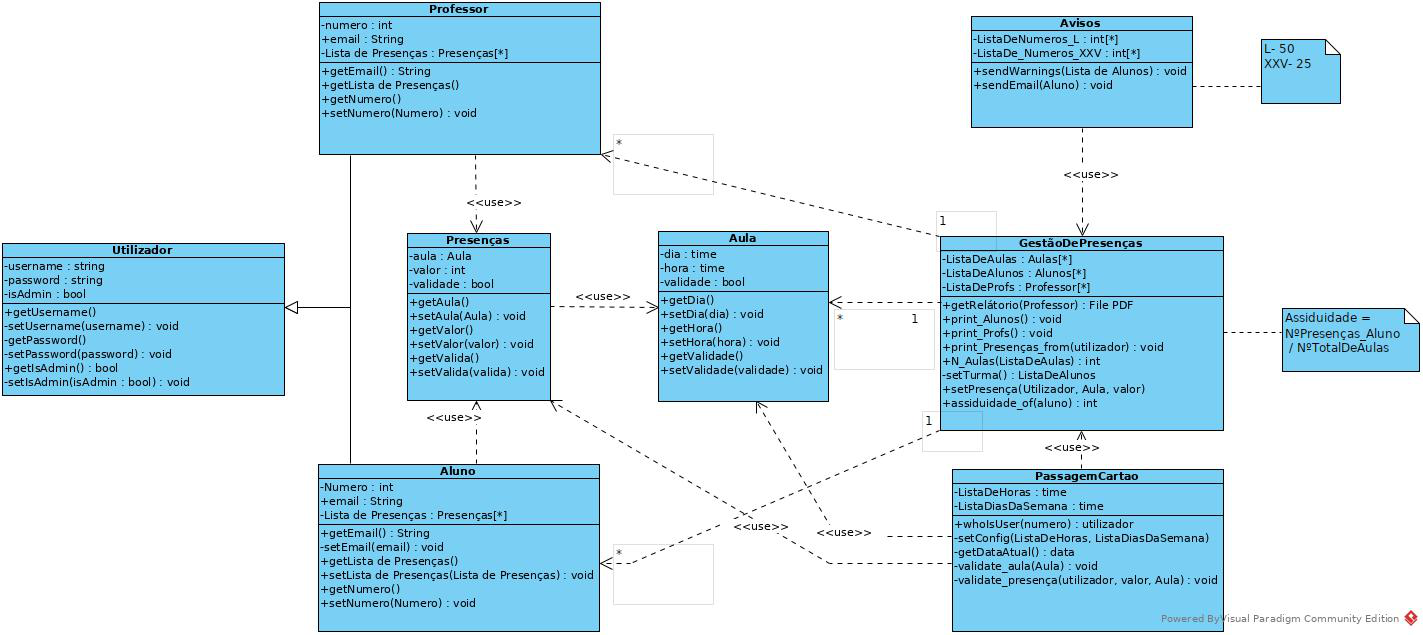
\includegraphics[width=\textwidth]{images/diagrama_classes.png}

\subsection{Diagramas de Atividades}

\subsubsection{Passagem Cartão}
    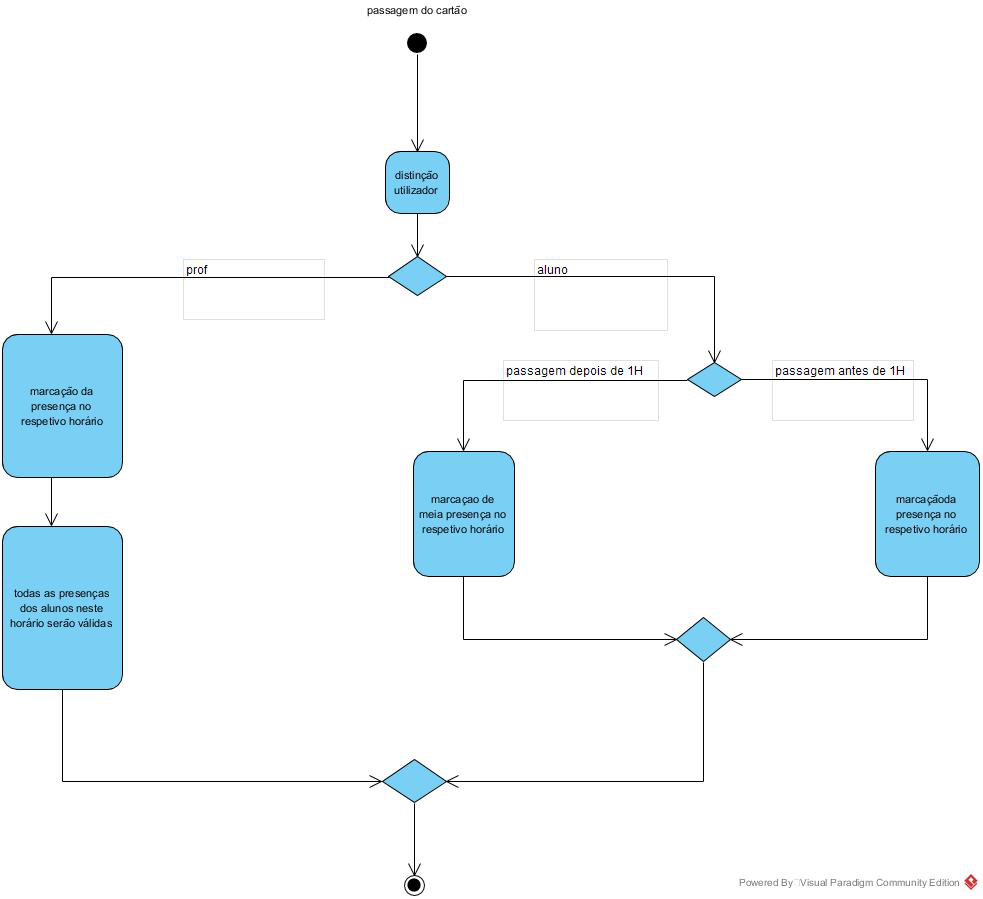
\includegraphics[width=\textwidth]{images/diagrama_atividades_cartao.png}

\subsubsection{Aviso de Faltas}
    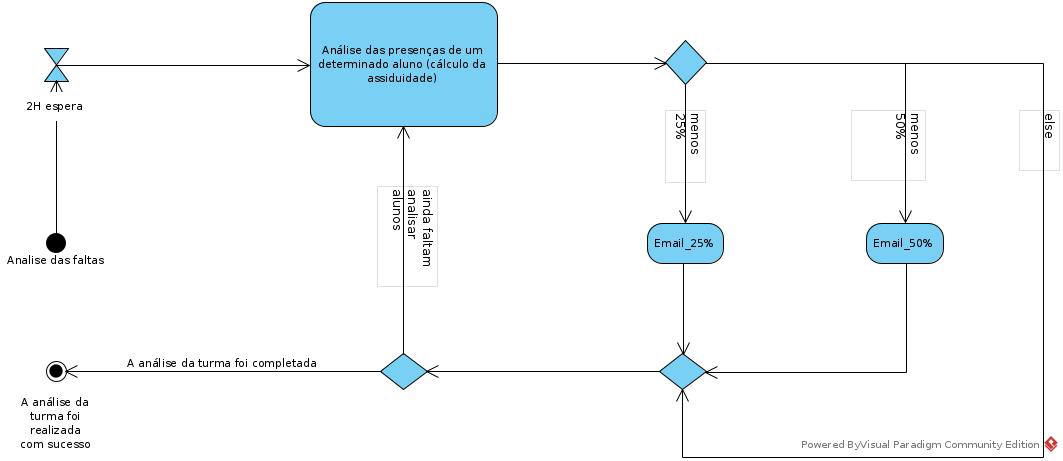
\includegraphics[width=\textwidth]{images/diagrama_atividades_faltas.png}

% -------------------------------------------------------------------------------------------
\newpage
\section{Conclusão} % Conclusão
\hspace{0,5cm}Em suma, com a realização deste trabalho "Simulador de Escalonamento" fiquei muito mais esclarecido sobre o seu funcionamento. \par
Saliento que me ajudou a entender como funciona o escalonador e as condições que cada algoritmo (\textbf{FCFS}/\textbf{RR}), usa para proceder à mudança dos processos entre os estados e as respetivas diferenças de tempo no mesmo conjunto de processos, entre os respetivos algoritmos.  
% -------------------------------------------------------------------------------------------
\end{document}